
\chapter{復習と補足}
\section{群論の復習と補足}
\subsection{群論や代数の復習}
授業で取り上げるのは幾何学的な群論であるが，群論の一般論から分かることも多いのでここに簡単に群論や代数の初等的な概念や結果を纏めておくので参考にしてほしい．

%$H\subset G$が\term[]{部分群}とは$H$が$G$の積に関して群となることである．これは
%\[
%     a,b\in H\Rightarrow ab\in H\quad\text{かつ}\quad 
%     a\in H\Rightarrow a^{-1}\in H
%\]
%を満たすことと同値である．

群$G$, $H$ について写像$f:G\to H$が
\[
     f(ab)=f(a)f(b)\quad \forall a,b\in G
\]
をみたすとき，$f$を\term[]{準同形}写像という．
$e_G$を$G$の単位元とすると
\[
     f(e_G)=e_H, \quad f(a^{-1})=f(a)^{-1} 
\]
が成り立つ．
特に準同形$f:G\to H$が全単射である
（自然に逆写像も準同形になる）とき
\term[]{同形}という．
準同形$f:G\to H$に対して
\[
     \Image f =\{f(a)\in H\mid a\in G\},\quad
      \Ker f=\{a\in G\mid f(a)=e\}
 \]
 と置くと，$\Image f$は$H$の部分群，$\Ker f$も$G$の部分群である．

群$G$の部分群$H$が与えられたとき，$g\in G$に対して
\[
     gH=\{gh\mid h\in H\},\quad Hg=\{hg,\mid h\in H\}
     \subset G
\]
と置き
\[
     G/H = \{gH\mid g\in G\}
\]
とする．$G$が有限群の時
\[
     |G : H|= |G/H|
\]
と書き$H$の$G$における\term[]{指数}という．
\begin{Thm}
   有限群$G$の部分群$H$に対して
   \[
        |G| =|G : H| |H|
   \]
\end{Thm}

一般には$gH\neq Hg$であるが，
\[
     \text{任意の}\quad g\in G\quad\text{に対して}\quad gH= Hg
\]
が成り立つとき$H$は$G$の\term[]{正規部分群}という．これは
\[
     \text{任意の}\quad g\in G\quad\text{に対して}\quad gHg^{-1}= H
\]
と同値である．$H\lhd G$と書くことがある．
$N$が$G$の正規部分群とするとき
\[
     G/N = \{gN\mid g\in G\}
\]
と置く．正規部分群の定義より
\[
     gNhN
     =g(hh^{-1})NhN
     =gh(h^{-1}Nh)N=gh NN =gh N
\]
特に
\[
     g^{-1}NgN=g^{-1}gN=N
\]
となり，$G/N$も群になる．これを\term[]{剰余群}という．%商群

$f:G\to H$を準同形とすると，$a\in\Ker f$,  $g\in G$に対して
\[
     f(gag^{-1})=f(g)f(a)f(g^{-1})=f(g)ef(g)^{-1}=f(g)f(g)^{-1}=e
\]
なので$\Ker f$は$G$の正規部分群である．このとき
\[
     G/\Ker f\sim \Image f
\]
が成り立つというのが群の\term[]{準同形定理}であった．
\emptyline

$\mathbf N$ を（$1$以上の）自然数全体のなす集合, $\mathbf Z$を整数全体のなす集合とする．$\mathbf Z$は加法$+$に関して群である．
$\mathbf Z$には掛け算$\cdot$ ( $\times$と書くこともある)もあるが$0$を除いた$\mathbf Z\setminus\{0\}$では割り算ができないこともあるので群ではない．
つまり，$\mathbf Z$は$+$と$\cdot$ に関して環であるが，体\footnote{環$K$の$0$以外の元が$\cdot$についての逆元を持つこと}ではない．

$m+n=n+m$なので可換群（アーベル群）である，加法$+$に関して加群ということがある．
$m\in \mathbf N$を固定し，$x, x'\in \mathbf Z $
\[
     x\equiv x' \mod m \Leftrightarrow 
     \exists q \in  \mathbf Z \text{ such that }x-x'=qm
\]
と置くとこれは同値関係である．
$x\in \mathbf Z $を代表元とする同値類を$\bar x$と置く．
%$\mathbf Z $を加法$+$に関する可換群と見なすと
\[
\begin{split}
     &x\equiv x' \mod m  \text{ and } y\equiv y' \mod m\\
     \Rightarrow \quad
     & x + y \equiv x' + y' \mod m,\quad
     xy\equiv x'y' \mod m
\end{split}
\]
なので
\[
     \bar x + \bar y = \overline{x+y},\quad
     \bar x\cdot \bar y = \overline{xy}
\]
と定め暫く$G$と置く．
$(G, +)$ は$\bar 0$を単位元とする可換群である．
\[
     f:\mathbf Z \ni x \to \bar x \in G
\]
とすると
\[
     \Ker f= m\mathbf Z=\bar 0
\]
見なせる．
$ m\mathbf Z$は$\mathbf Z$の正規部分群であるので，準同形定理より
\[
     G \sim \mathbf Z/m\mathbf Z
\]
となる．
\term[]{巡回群}とは一つの元から生成される群のことであった．$\mathbf Z/m\mathbf Z$は$\bar 1$で生成されているので有限巡回群である．授業では回転で生成される有限部分群を巡回群といったが，普通はこちらの定義の方が一般的である．例えば$D_1$も巡回群で$C_2$と同形である．
また，無限集合になる巡回群を無限巡回群というが
無限巡回群は$\mathbf Z$と同形になる．
\emptyline

以下，
$\mathbf Z/m\mathbf Z$の積$\cdot$についての構造を調べる．
最初にいくつか計算してみる．

\begin{ex}
   $\mathbf Z/4\mathbf Z$の足し算と掛け算の演算表を作ってみる．
   足し算については巡回群$C_4$なのでそのままであるが，
   積に関しては$\bar 2$が零因子となっているので群でなく，
   従って$\mathbf Z/4\mathbf Z$は体でない．
   \begin{table}[htb]
      \centering
      \begin{minipage}{0.4\columnwidth}
           \centering
           \begin{tabular}{l|llll}
                 $+$&$\bar 0$&$\bar1$&$\bar2$&$\bar3$ \\ \hline
                $\bar 0$&$\bar 0$&$\bar1$&$\bar2$&$\bar3$ \\
                $\bar1$& $\bar1$&$\bar2$ &$\bar3$&$\bar0$ \\
                $\bar2$ &$\bar2$&$\bar3$&$\bar 0$&$\bar1$ \\ 
                $\bar3$& $\bar3$ &$\bar0$& $\bar1$&$\bar2$\\ 
           \end{tabular}
           \caption{$+$ $\mod 4$}\label{mod4plus}
      \end{minipage} 
      \begin{minipage}{0.4\columnwidth}
           \centering
           \begin{tabular}{l|llll}
                 $\cdot$&$\bar 0$&$\bar1$&$\bar2$&$\bar3$ \\ \hline
                $\bar 0$&$\bar 0$&$\bar0$&$\bar0$&$\bar0$ \\
                $\bar1$& $\bar0$&$\bar1$ &$\bar2$&$\bar3$ \\
                $\bar2$ &$\bar0$&$\bar2$&$\bar 0$&$\bar2$ \\ 
                $\bar3$& $\bar0$ &$\bar3$& $\bar2$&$\bar1$\\ 
           \end{tabular}
           \caption{$\cdot$ $\mod 4$}\label{mod4times}
      \end{minipage} 
   \end{table}
\end{ex}

\begin{ex}
   $\mathbf Z/5\mathbf Z$の足し算と掛け算の演算表を作ってみる．
   掛け算では零因子がないので$\bar0$を除く$(\mathbf Z/5\mathbf Z)^{\times}=(\mathbf Z/5\mathbf Z)\setminus \{\bar 0\}$は群となる．
   これは巡回群$C_4$と同型である(表~\ref{mod4plus}
   と異なって見えるかもしれないが，$\bar 1_4$, $\bar 2_5$のように表し区別し，$\varphi:(\mathbf Z/5\mathbf Z)^{\times}\to \mathbf Z/4\mathbf Z$を
   \[
        \varphi(\bar 1_5)=\bar 0_4,\quad
        \varphi(\bar 2_5)=\bar 1_4,\quad
        \varphi(\bar 3_5)=\bar 3_4,\quad
        \varphi(\bar 4_5)=\bar 2_4
   \]
   とすると$(\mathbf Z/5\mathbf Z)^{\times}$は掛け算，$\mathbf Z/4\mathbf Z$は足し算として同型になることが分かる)．
   このことから$\mathbf Z/5\mathbf Z$は体でもある．
   
   \begin{table}[htb]
      \centering
      \begin{minipage}{0.4\columnwidth}
           \centering
           \begin{tabular}{l|lllll} 
                 $+$&$\bar 0$&$\bar1$&$\bar2$&$\bar3$ &$\bar4$\\ \hline
                $\bar 0$&$\bar 0$&$\bar1$&$\bar2$&$\bar3$&$\bar4$ \\
                $\bar1$& $\bar1$&$\bar2$ &$\bar3$&$\bar4$& $\bar0$\\
                $\bar2$ &$\bar2$&$\bar3$&$\bar 4$&$\bar0$&$\bar1$ \\ 
                $\bar3$& $\bar3$ &$\bar4$& $\bar0$&$\bar1$&$\bar2$\\ 
                $\bar4$& $\bar4$& $\bar0$&$\bar1$&$\bar2$&$\bar2$ \\
           \end{tabular}
           \caption{$+$ $\mod 5$}
      \end{minipage} 
      \begin{minipage}{0.4\columnwidth}
           \centering
           \begin{tabular}{l|lllll} 
                 $\cdot$&$\bar 0$&$\bar1$&$\bar2$&$\bar3$ &$\bar4$\\ 
                \hline
                $\bar 0$&$\bar 0$&$\bar0$&$\bar0$&$\bar0$&$\bar0$ \\
                $\bar1$& $\bar0$&$\bar1$ &$\bar2$&$\bar3$ &$\bar4$\\
                $\bar2$ &$\bar0$&$\bar2$&$\bar 4$&$\bar1$ &$\bar3$\\ 
                $\bar3$& $\bar0$ &$\bar3$& $\bar1$&$\bar4$&$\bar2$\\ 
                $\bar4$& $\bar0$& $\bar4$&$\bar3$&$\bar2$&$\bar1$ \\
           \end{tabular}
           \caption{$\cdot$ $\mod 5$}
      \end{minipage} 
   \end{table}
\end{ex}

%上で指摘したように$\mathbf Z/m\mathbf Z$には$\cdot$という積があり環となっている．しかし，$\bar 0$を除いても$\cdot$に関して一般には群ではない．


$m, n\in \mathbf Z$に対して$(m,n)$で$m$ と $n$の最大公約数を表す．
\[
     (m,n)=1
     \quad \Leftrightarrow\quad
     \exists a, b\in \mathbf Z \text{ such that } am + bn =1
\]
がユークリッドの互除法から分かる．このことから
\[
     (m,n)=1
     \quad \Leftrightarrow\quad
     \exists  \bar b\in \mathbf Z/m\mathbf Z \text{ such that } 
           \bar b\bar n= \bar 1
\]
$m\in \mathbf N$を固定し$(m,n)=1$なる
$\bar n\in\mathbf Z/m\mathbf Z$を\term[]{既約剰余類}という．
既約剰余類$\bar a\in \mathbf Z/m\mathbf Z$ を固定すると$\bar b\bar a = \bar 1$なる$\bar b\in \mathbf Z/m\mathbf Z$が見つかるので
\[
     f:\mathbf Z/m\mathbf Z\ni \bar n 
      \mapsto \bar{a}\cdot\bar{n}\in  \mathbf Z/m\mathbf Z
\]
を考えると$f$は$+$に関して準同形写像で，$\bar b$を掛けることで同形写像であることが分かる．
\[
     \varphi(m)= |\{n\mid n=1,\dots, m \text{ such that } (m,n)=1\}|
\]
と置くと$\mathbf Z/m\mathbf Z$には$\varphi(m)$個の既約剰余類が存在することが分かる．$\varphi$はオイラー関数と言われる．
したがって$\mathbf Z/m\mathbf Z$には$\varphi(m)$個の生成元が存在し，$\mathbf Z/m\mathbf Z$はどの生成元をとっても加群としては
同型な巡回群となる．

$(m,n)=1$なる$n$を固定する．
$x_1, \cdots, x_{\varphi(m)}$を$\mathbf Z/m\mathbf Z$の既約剰余類全体とする．$\bar n x_1, \cdots , \bar nx_{\varphi(m)}$も既約剰余類全体なので，集合としては一致している．したがって
\[
     x_1\cdots x_{\varphi(m)}=\bar n x_1 \cdots \bar n x_{\varphi(m)}
     =\bar n^{\varphi(m)}x_1\cdots x_{\varphi(m)}
\]
$x_1, \cdots , x_{\varphi(m)}$は逆元をもつので
$
     \bar n^{\varphi(m)}=\bar 1\in\mathbf Z/m\mathbf Z
$,  つまり
\[
     n^{\varphi(m)}\equiv 1 \mod m
\]
$p$を素数とすると，$\varphi(p)=p-1$なので任意の$x\not\equiv 0 \mod p$に対して
\[
     x^{p-1}\equiv 1 \mod p
\]
となり，\term[]{フェルマーの小定理}が得られる．これから任意の$x\in \mathbf Z$に対して
\begin{equation}\label{funPoly}
     x^{p}\equiv x \mod p
\end{equation}
も分かる．
フェルマーの小定理は$(\mathbf Z/p\mathbf Z)^{\times}=(\mathbf Z/p\mathbf Z)\setminus \{\bar 0\}$が積$\cdot$について巡回群であることを意味している．
特に$\mathbf Z/p\mathbf Z$が体であることも意味していている．
このとき$\mathbf F_p$と表すことが多い．これは標数$p$の有限体である．

\begin{Quiz}
   標数$p$の有限体は$\mathbf F_p$の有限次元拡大であること，
   それが$\mathbf F_p$のガロワ拡大であることを示し，
   そのガロワ群を決定せよ（ヒント$:$
    \eqref{funPoly}の形の多項式でガロワ拡大を特徴付けよ）．
\end{Quiz}



\subsection{アミダクジと置換群}
最初に置換と阿弥陀籤が同じものであることを示す．
アミダクジの例を次にあげる．
\begin{figure}[htb]
     \centering
     \includegraphics{~/Documents/GitHub/bEuclideanGeo/appa/images/figure09.1}
     \caption{アミダクジ $\tau$}\label{}
\end{figure}
$4$本の柱に順に$1,\dots,4$と名前を付け，そのアミダクジを上から下にたどるとき何番目の柱から何番目の柱に移るかのリストと同一視することにする．例えば．このアミダクジでは柱$1$から柱$2$に移り，柱$2$から柱$4$に移り，柱$3$から柱$1$に移り，柱$4$から柱$3$に移るので，このアミダクジを
$\begin{pmatrix}1&2&3&4\\2&4&1&3\end{pmatrix}$と表す．
これを置換（表示）ということもある．
上の数字は上の柱の番号で対になる下の番号が移る柱の番号を表している．下の行に出てくる数字に重複がないことを確かめてほしい．
簡単のため，このアミダクジを$\tau$と表す．
\[
     \tau(1)=2, \tau(2)=4,\tau(3)=1,\tau(4)=3
\]
と表すこともある．つまり，アミダクジ$\tau$は$\{1,2,3,4\}$から$\{1,2,3,4\}$への上への一対一対応（写像）を定めている．

アミダクジ$\rho$を
\begin{figure}[htb]
     \centering
     \includegraphics{~/Documents/GitHub/bEuclideanGeo/appa/images/figure09.2}
     \caption{アミダクジ $\rho$}\label{}
\end{figure}

\noindent
とする．$\tau$を行ったあと$\rho$を行う事によって出来るアミダクジ
\vspace{10pt}

\begin{figure}[htb]
     \centering
     \includegraphics{~/Documents/GitHub/bEuclideanGeo/appa/images/figure09.3}
     \caption{$\tau$と$\rho$の合成}\label{}
\end{figure}

\noindent
を$\tau$と$\rho$の\term[]{積}(\term[]{掛け算})といい，$\rho\tau$と表す．つまり，対応（写像）としては
\[
     \rho\tau(i)=\rho(\tau(i))\qquad i=1,2,3,4
\]
（つまり，関数の合成や，(ベクトルを作用させた)行列の積と同じ）である．置換を使い
\[
     \rho\tau
     =
     \begin{pmatrix}1&2&3&4\\ 4&2&1&3\end{pmatrix}
     \begin{pmatrix}1&2&3&4\\2&4&1&3\end{pmatrix}
     =
     \begin{pmatrix}1&2&3&4\\2&3&4&1\end{pmatrix}
\]
のように$\tau$で$1$が$2$にうつり，次に$\rho$で$2$が$2$にうつるので$\rho\tau$では$1$が$2$うつる，$\tau$で$2$が$4$にうつり，次に$\rho$で$4$が$3$にうつるので$\rho\tau$では$2$が$4$うつる
というように計算してもいい．

\begin{Quiz}
\[
     \tau\rho=
     \begin{pmatrix}1&2&3&4\\2&4&1&3\end{pmatrix}
     \begin{pmatrix}1&2&3&4\\ 4&2&1&3\end{pmatrix}
     =
     \begin{pmatrix}1&2&3&4\\ & & & \end{pmatrix}
\]
の空白を埋め，$\tau\rho\neq\rho\tau$を確かめよ．
\end{Quiz}

順番を変えないアミダクジを\term[]{単位}アミダクジといい，$\varepsilon$と表す．つまり，
\begin{figure}[htb]
     \centering
     \includegraphics{~/Documents/GitHub/bEuclideanGeo/appa/images/figure09.4}
     \caption{単位アミダクジ}\label{}
\end{figure}

明らかに任意のアミダクジ$\sigma$に対して
\[
     \varepsilon\sigma=\sigma\varepsilon=\sigma
\]
が成り立つ．

アミダクジ$\sigma$を下から上にたどって出来るアミダクジを\term[]{逆}アミダクジといい，$\sigma^{-1}$と表す．例えば$\tau$の逆は

\begin{figure}[htb]
     \centering
     \includegraphics{~/Documents/GitHub/bEuclideanGeo/appa/images/figure09.5}
     \caption{逆アミダクジ}\label{}
\end{figure}

\noindent
である．左側では置換表示の上の行と下の行を入れ替え，それを並び替えるという操作を行っている．
さらに
\begin{figure}[htb]
     \centering
     \includegraphics{~/Documents/GitHub/bEuclideanGeo/appa/images/figure09.6}
     \caption{アミダクジと逆アミダクジの合成}\label{}
\end{figure}

\noindent
これは行った道を逆にたどれば元いた場所に戻れるということをアミダクジで表しただけなので，任意のアミダクジ$\sigma$に対して
\[
     \sigma^{-1}\sigma=\sigma\sigma^{-1}=\varepsilon
\]
が成り立つ．このようにアミダクジの積はアミダクジの自然な演算を与えている．
\emptyline

$n$本のアミダクジ$\sigma$は
$\{1,2,3,\dots,n\}$から$\{1,2,3,\dots,n\}$への上への一対一対応（写像）
\[
      \sigma=
     \begin{pmatrix}
          1&2&3&\cdots&n\\
          i_1&i_2&i_3&\cdots&i_n
     \end{pmatrix}
\]
で表せる．ただし，$\{i_1,i_2,i_3,\cdots,i_n\}=\{1,2,3,\dots,n\}$ である．
このような写像を$n$\term[]{次置換}という．
同じ置換を表すアミダクジを合同ということにする．
逆に，一般の$n$次置換が$n$本の（ある合同な）アミダクジで表せるかという問題を考えよう．


次のようなアミダクジ（置換）を考える：
\begin{figure}[htb]
     \centering
     \includegraphics{~/Documents/GitHub/bEuclideanGeo/appa/images/figure09.7}
     \caption{循環置換}\label{}
\end{figure}

\noindent
このような置換を（4次の）\term[]{循環置換}といい，
$\begin{pmatrix}1&2&3&4\end{pmatrix}$と表す．
特に$2$次の循環置換を\term[]{互換}という．
例えば

\begin{figure}[htb]
     \centering
     \includegraphics{~/Documents/GitHub/bEuclideanGeo/appa/images/figure09.8}
     \caption{互換}\label{}
\end{figure}

\noindent
である．
上の巡回置換を次のように点線で分けて考えると
\begin{figure}[htb]
     \centering
     \includegraphics{~/Documents/GitHub/bEuclideanGeo/appa/images/figure09.9}
     \caption{アミダクジの互換への分解}\label{}
\end{figure}

\noindent
が成り立つ．
右から左の積の順番はアミダクジの上から下への連結に対応していることをあらためて注意しておく．
また，
別やり方で表すと
\begin{figure}[htb]
     \centering
     \includegraphics{~/Documents/GitHub/bEuclideanGeo/appa/images/figure09.12}
     \caption{アミダクジの互換への別の分解}\label{}
\end{figure}

\noindent
のようになる．
このように置換のアミダクジによる表し方は色々あるので，覚えやすい方法で覚え，わからくなったらアミダクジで表してみることをお奨めする．次に



\begin{figure}[h]
     \centering
     \includegraphics{~/Documents/GitHub/bEuclideanGeo/appa/images/figure09.10}
     \caption{互換のアミダクジでの表示}\label{}
\end{figure}

\noindent
のように任意の柱の互換もアミダクジで表すことが出来る．

\begin{comment}
以上より
循環置換$\begin{pmatrix}i_1&i_2&\dots&i_r\end{pmatrix}$は
\begin{figure}[htb]
     \centering
     \includegraphics{~/Documents/GitHub/bEuclideanGeo/appa/images/figure09.11}
\end{figure}
と互換の積に分解される．
\end{comment}

以上の準備のもと，一般の置換は互換の積で表せることを例を使って示す．
\begin{exQ} 次の置換を循環置換の積に分解し，更に互換の積で表せ．
\[
     \mu=
     \begin{pmatrix}
          1&2&3&4&5&6&7\\
          4&1&6&2&7&5&3
     \end{pmatrix}
\]
\end{exQ}
解答）
$1$が$4$に移り，$4$が$2$に移り，$2$が$1$に移ので，
巡回置換$\begin{pmatrix}1&4&2\end{pmatrix}$になっている．
\[
\begin{split}
     \mu&\Rightarrow 
     \begin{pmatrix}
          1&2&3&4&5&6&7\\\downarrow&&&&&&\\
           4&1&6&2&7&5&3 
      \end{pmatrix}\\
     &\Rightarrow 
     \begin{pmatrix}
          1&2&3&4&5&6&7\\
          \downarrow&&&\downarrow&&&\\
           4&1&6&2&7&5&3 
      \end{pmatrix}\\
     &\Rightarrow 
     \begin{pmatrix}
          1&2&3&4&5&6&7\\
          \downarrow&\downarrow&&\downarrow&&&\\
           4&1&6&2&7&5&3 
      \end{pmatrix}\\
     &\Rightarrow \begin{pmatrix}1&4&2\end{pmatrix}
\end{split}
\]
残りをみると
$3$が$6$に移り，$6$が$5$に移り，$5$が$7$に移り，$7$が$3$に移
ので，巡回置換$\begin{pmatrix}3&6&5&7\end{pmatrix}$になっている．
\[
\begin{split}
     \mu&=\begin{pmatrix}1&2&3&4&5&6&7\\\downarrow&\downarrow&\Downarrow&\downarrow&\Downarrow&\Downarrow&\Downarrow\\
      4&1&6&2&7&5&3 \end{pmatrix}\\
     &=\begin{pmatrix}1&4&2\end{pmatrix}
     \begin{pmatrix}3&6&5&7\end{pmatrix}
\end{split}
\]
したがって，先程のように巡回置換を互換で表すと
\[
\begin{split}
     \mu&=\begin{pmatrix}1&4&2\end{pmatrix}
     \begin{pmatrix}3&6&5&7\end{pmatrix}\\
     &=\begin{pmatrix}1&4\end{pmatrix}
     \begin{pmatrix}4&2\end{pmatrix}
     \begin{pmatrix}3&6\end{pmatrix}
     \begin{pmatrix}6&5\end{pmatrix}
     \begin{pmatrix}5&7\end{pmatrix}.
\end{split}
\]
もちろん
\[
\begin{split}
     \mu&=
     \begin{pmatrix}3&6&5&7\end{pmatrix}
     \begin{pmatrix}1&4&2\end{pmatrix}
     \\
     &=
     \begin{pmatrix}3&6\end{pmatrix}
     \begin{pmatrix}6&5\end{pmatrix}
     \begin{pmatrix}5&7\end{pmatrix}
     \begin{pmatrix}1&4\end{pmatrix}
     \begin{pmatrix}4&2\end{pmatrix}.
\end{split}
\]
でも構わない．

以上のやり方で全ての置換は互換の積で表せることが分かり，
全ての置換はアミダクジで表される．つまり，置換とアミダクジは同じものであることが分かる．

\emptyline
最後に$\sigma$が$m$個の互換の積にかける(つまり，アミダクジの横棒が$m$本の)とき
\[
     \sign \sigma=(-1)^m
\]
で$\sigma$の\term[]{符号}を定める．例えば上の$\mu$については$\sign\mu=(-1)^5=-1$である．
%また，最初の例の$\rho$ではもともとアミダクジで表されていて，互換の数（つまり，横の線の数）は$4$個なので，$\sign\tau=1$である．
\begin{exQ}  次の置換を互換の積で表し，符号を求めよ．
\[
     \mu=\begin{pmatrix}
          1&2&3&4&5&6&7&8&9\\
          7&6&8&2&1&4&9&3&5
     \end{pmatrix}
\]
\end{exQ}
解答）
\[
\begin{split}
     \mu&=
     \begin{pmatrix}
          1&7&9&5
     \end{pmatrix}
     \begin{pmatrix}
          2&6&4
     \end{pmatrix}
     \begin{pmatrix}
          3&8
     \end{pmatrix}\\
     &=\begin{pmatrix}
          1&7
     \end{pmatrix}
     \begin{pmatrix}
          7&9
     \end{pmatrix}
     \begin{pmatrix}
          9&5
     \end{pmatrix}
     \begin{pmatrix}
          2&6
     \end{pmatrix}
     \begin{pmatrix}
          6&4
     \end{pmatrix}
     \begin{pmatrix}
          3&8
     \end{pmatrix}
\end{split}
\]
よって，$\sign \mu=(-1)^6=1$.
\emptyline

単位置換$\varepsilon$は$0$個の互換の積であらわせるので
\[
     \sign\varepsilon=(-1)^0=1
\]
また，定義から
\[
     \sign \sigma\tau=\sign \sigma\sign \tau,\quad \sign \sigma^{-1}= \sign \sigma
\]
が成り立つ．
$\sign \sigma=1$のとき$\sigma$を\term[]{偶置換}，
$\sign \tau=-1$のとき$\tau$を\term[]{奇置換}という．
特に，$\sign:S_n\to \{1, -1\}$は準同形写像であり，
$A_n = \Ker \sign =\{\sigma\in S_n\mid $偶置換$\}$は部分群である．

%\[
%     \mu=\begin{pmatrix}1&2&3&4&5&6&7&8\\4&8&6&3&1&5&2&7\end{pmatrix}
%\]
%とすると，$1$が$4$に移り，$4$が$3$に移り，$3$が$6$に移り，$6$が$5$に移り，$5$が$1$に移ので，巡回置換$\begin{pmatrix}1&4&3&6&5\end{pmatrix}$になっている．残りをみると
%$2$が$8$に移り，$8$が$7$に移り，$7$が$2$に移る
%ので，巡回置換$\begin{pmatrix}2&8&7\end{pmatrix}$になっている．したがって，先程のように巡回置換を互換で表すと
%\[
%\begin{split}
%     \mu&=\begin{pmatrix}1&4&3&6&5\end{pmatrix}\begin{pmatrix}2&8&7\end{pmatrix}\\
%     &=\begin{pmatrix}1&4\end{pmatrix}
%     \begin{pmatrix}4&3\end{pmatrix}
%     \begin{pmatrix}3&6\end{pmatrix}
%     \begin{pmatrix}6&5\end{pmatrix}
%     \begin{pmatrix}2&8\end{pmatrix}
%     \begin{pmatrix}8&7\end{pmatrix}
%\end{split}
%\]
%もちろん数字の大きい方から始めて
%\[
%\begin{split}
%     \mu&=\begin{pmatrix}8&7&2\end{pmatrix}\begin{pmatrix}6&5&1&4&3\end{pmatrix}\\
%     &=
%     \begin{pmatrix}8&7\end{pmatrix}
%     \begin{pmatrix}7&2\end{pmatrix}
%     \begin{pmatrix}6&5\end{pmatrix}
%     \begin{pmatrix}5&1\end{pmatrix}
%     \begin{pmatrix}1&4\end{pmatrix}
%     \begin{pmatrix}4&3\end{pmatrix}
%\end{split}
%\]
%でも構わない．


\begin{Quiz}
　次の置換を互換の積に表せ．
   \[
        \begin{pmatrix}
             1&2&3&4&5\\
             4&5&2&1&3
        \end{pmatrix}
   \]
   それを用いて，この置換を表すアミダクジを一つ作れ．
\end{Quiz}

\subsection{置換群と交代群の構造}
$n$次置換群の構造を調べる．
$n$次の置換全体を$S_n$と置く．$S_n$は群であり，$n$\term[]{次置換群}と呼ばれる．
$S_n$の元は$\begin{pmatrix}1&2&3&\cdots&n\\i_1&i_2&i_3&\cdots&i_n\end{pmatrix}$と表されるので，個数は$n!$ である．これがアミダクジで表されるので，$S_n$は$n-1$個の互換$\begin{pmatrix}1&2\end{pmatrix}$, $\begin{pmatrix}2&3\end{pmatrix}$, \dots, $\begin{pmatrix}n-1&n\end{pmatrix}$
により生成されることが分かる．

$A_n=\{\sigma\in S_n\mid$ 偶置換 $\}$と置くと
 \begin{gather*}
      \sigma,\tau\in A_n
     \Rightarrow
     \sign \sigma\tau=\sign \sigma  \sign\tau=1
     \Rightarrow
      \sigma\tau\in A_n
     \\
       \sigma\in A_n
     \Rightarrow 
     \sign \sigma^{-1}=\sign \sigma=1
     \Rightarrow
     \sigma^{-1}\in A_n
 \end{gather*}
 が成り立つので$A_n$は$S_n$の{部分群}であり，$n$\term[]{次交代群}と呼ばれる．
 \emptyline

 $n=3$のとき$S_3$は
\begin{equation}
\begin{split}
   \begin{pmatrix}1&2&3\\1&2&3\end{pmatrix}=\varepsilon,\quad
   \begin{pmatrix}1&2&3\\1&3&2\end{pmatrix}
   =
   \begin{pmatrix}
      2&3
   \end{pmatrix},\\
   \begin{pmatrix}1&2&3\\2&1&3\end{pmatrix}
   =\begin{pmatrix}
      1&2
   \end{pmatrix},\quad
   \begin{pmatrix}1&2&3\\2&3&1\end{pmatrix}
   =\begin{pmatrix}
      1&2&3
   \end{pmatrix},\\
   \begin{pmatrix}1&2&3\\3&1&2\end{pmatrix}=
   \begin{pmatrix}
      1&3&2
   \end{pmatrix},\quad
   \begin{pmatrix}1&2&3\\3&2&1\end{pmatrix}=
   \begin{pmatrix}
      1&3
   \end{pmatrix}
\end{split}\label{S3}
\end{equation}
の$3!=6$個からなり，$\varepsilon$, $\begin{pmatrix}
          1&2&3
     \end{pmatrix}$, $\begin{pmatrix}
          1&3&2
     \end{pmatrix}$が偶置換で，$\begin{pmatrix}
          1&2
     \end{pmatrix}$, $\begin{pmatrix}
          2&3
     \end{pmatrix}$, $\begin{pmatrix}
          1&3
     \end{pmatrix}$が奇置換である．
よって
\[
     A_3 = \{
     \varepsilon, 
     \begin{pmatrix}
          1&2&3
     \end{pmatrix},
     \begin{pmatrix}
          1&3&2
     \end{pmatrix} \}\subset S_3
\]
で$A_3$は$C_3$と同形．
\emptyline

次に$n=4$のとき
 \[
\begin{split}
     K=\{\varepsilon, &\quad
     \alpha=\begin{pmatrix}1&2\end{pmatrix}
     \begin{pmatrix}3&4\end{pmatrix}, \quad
     \beta=\begin{pmatrix}1&3\end{pmatrix}
     \begin{pmatrix}2&4\end{pmatrix},\\
     &\gamma=\begin{pmatrix}1&4\end{pmatrix}
     \begin{pmatrix}2&3\end{pmatrix}\}
     \subset  A_4
\end{split}
\]
\begin{figure}[thb]
     \centering
     \includegraphics{~/Documents/GitHub/bEuclideanGeo/ch1/figureGroup3.7}
     \caption{$\alpha$, $\beta$, $\gamma$}
\end{figure}


\noindent
とすると，明らかに$\alpha^2=\beta^2=\gamma^2=\varepsilon$で，
図 \ref{betaAlphaGamma}より
\[
     \alpha\beta=\beta\alpha=\gamma
\]

\begin{figure}[htb]
     \centering
     \includegraphics{~/Documents/GitHub/bEuclideanGeo/ch1/figureGroup3.8}
     \caption{$\beta\alpha=\gamma=\alpha\beta$}\label{betaAlphaGamma}
\end{figure}

\noindent
これから
\[
     \gamma\alpha=\beta\alpha\alpha=\beta,\quad
     \alpha\gamma=\alpha\alpha\beta=\beta
\]
のように計算することで次の表を得る．

\begin{table}[htb]
      \centering
      \begin{tabular}{l|llll}\noalign{\hrule height 1pt}
         &$\varepsilon$&$\alpha$&$\beta$&$\gamma$ \\ 
         \hline
         $\varepsilon$&$\varepsilon$&$\alpha$&$\beta$&$\gamma$ \\
         $\alpha$& $\alpha$&$\varepsilon$ &$\gamma$&$\beta$ \\
         $\beta$& $\beta$&$\gamma$&$\varepsilon$&$\alpha$ \\ 
         $\gamma$& $\gamma$ &$\beta$&  $\alpha$&$\varepsilon$\\
        \noalign{\hrule height 1pt}
      \end{tabular}     \caption{クライン群$K$の演算表}
\end{table}

\noindent
$K$は$A_4$の部分群であり，積が順番によらないこともわかる．
$K$はクライン群と呼ばれる可換群である．以後
$\begin{pmatrix}1&2\end{pmatrix}\begin{pmatrix}3&4\end{pmatrix}$
等を独立な互換の積ということがある．

%\emptyline
%$G$を群，$H$を$G$の部分群とする．$g\in G$について
%一般には$gH\neq Hg$であるが，
%\[
%     \text{任意の}\quad g\in G\quad\text{に対して}\quad gH= Hg
%\]
%が成り立つとき$H$は$G$の\term[]{正規部分群}という．これは
%\[
%     \text{任意の}\quad g\in G\quad\text{に対して}\quad gHg^{-1}= H
%\]
%と同値である．$H\lhd G$と書くことがある．
$n$次交代群$A_n$は$S_n$の正規部分群である．なぜなら，任意の
$\sigma \in S_n$と$\tau\in A_n$に対して
\[
     \sign\sigma\tau\sigma^{-1}
     =\sign\sigma\sign\tau\sign\sigma^{-1}
     =\sign\tau=1
\]
なので$\sigma A_n\sigma^{-1}\subset A_n$, つまり，
$\sigma A_n\sigma^{-1}= A_n$となるからである．
\emptyline

%$H\lhd G$のとき正規部分群の定義より
%\[
%     gNhN
%     =g(hh^{-1})NhN
%     =gh(h^{-1}Nh)N=gh NN =gh N
%\]
%特に
%\[
%     g^{-1}NgN=g^{-1}gN=N
%\]
%となり，$G/N$も群になる．これを\term[]{商群}という．

群$G$について正規部分群の列
\[
     G_m=\varepsilon\lhd  G_{m-1}\lhd \cdots  \lhd G_1\lhd  G_0=G
\]
が存在し，その商群$G_{i-1}/G_{i}$が可換群であるとき$G$を
\term[]{可解群}という．ただし，$\varepsilon$ は単位元のみから成る群$\{\varepsilon\}$を意味する．

\emptyline
$S_3$では
\[
     \varepsilon\lhd   A_3 \lhd  S_3
\]
で，上で見たように
$ A_3$は$ S_3$の正規部分群で$S_3/ A_3$は可換群$C_2$であり，$A_3$は$\sigma=\begin{pmatrix}1&2&3\end{pmatrix}$で作られる$3$次循環群$C_3$であり可換群である．よって$S_3$は可解群である．
\emptyline

$S_4$は
\[
     \varepsilon\lhd  K\lhd  A_4 \lhd S_4
\]
という正規部分群の列を持つ．$K$は可換群で$ A_4$と$ S_4$部分は上と同じである．$\sigma\in S_n$はアミダクジ$\tau\in S_n$に$\sigma\tau\sigma^{-1}$で作用するが，これはアミダクジ$\tau$の柱の名前を付け替えることに対応している．$K$は二組の異なる柱の組の互換と単位置換からなるのでこの作用で保存される．したがって$K$は$A_4$の正規部分群であることが分かる．
$\sigma=\begin{pmatrix}1&2&3\end{pmatrix}\notin K$を固定すると，
$A_4/K=\{K, \sigma K, \sigma^{2}K\}$は$C_3$と同形となり，やはり可換群である．よって，$S_4$は可解群である．

\begin{Thm}
   $n\ge 5$のとき$A_n$は可解群でない．
\end{Thm}
\begin{proof}
   まず$A_n$の任意の元が$\begin{pmatrix}i&j&k\end{pmatrix}$の形の循環置換（以下，三環という）の積で表せることを示す．$A_n$は偶置換からなるので
   $\sigma=\begin{pmatrix}i&j\end{pmatrix}\begin{pmatrix}k&l\end{pmatrix}$
   の形($i\neq j$, $k\neq l$)の置換の積で表すことが出来る．
   $\{i,j\}=\{k,l\}$のときは$\sigma = \varepsilon$. 
   $\{i,j\}$と$\{k,l\}$の共通元が一個だけあるとき，それを$j=l$とすると
   \[
        \sigma =
        \begin{pmatrix}i&j\end{pmatrix}\begin{pmatrix}j&k\end{pmatrix}
        =\begin{pmatrix}i&j&k\end{pmatrix}
   \]
   $\{i,j\}$と$\{k,l\}$の共通元がないとき，
   \[
        \sigma =
        \begin{pmatrix}i&j\end{pmatrix}\begin{pmatrix}k&l\end{pmatrix}
        =\begin{pmatrix}i&j\end{pmatrix}\begin{pmatrix}j&k\end{pmatrix}
        \begin{pmatrix}j&k\end{pmatrix}\begin{pmatrix}k&l\end{pmatrix}
        =\begin{pmatrix}i&j&k\end{pmatrix}
        \begin{pmatrix}j&k&l\end{pmatrix}
   \]
   となるので証明できた．
   
   $A_n$の正規部分群$N\neq A_n$で$A_n/N$が可換群であるものが存在したとする．すると，任意の$g, h\in A_n$に対して
   \[
        ghN=gNhN=hNgN=hgN
   \]
   つまり，
   \[
        N= (gh)^{-1}hgN=h^{-1}g^{-1}hgN
   \]
   $\varepsilon\in N$より
   \[
        h^{-1}g^{-1}hg=h^{-1}g^{-1}hg\,\varepsilon\in N
   \]
   となる．
   
   
 \begin{figure}[thb]
      \centering
      \begin{minipage}{0.4\columnwidth}
         \centering
           \includegraphics{~/Documents/GitHub/bEuclideanGeo/ch1/figureGroup3.9}
           \caption{$h^{-1}g^{-1}hg$}
         \label{}
      \end{minipage} 
      \begin{minipage}{0.4\columnwidth}
         \centering
           \includegraphics{~/Documents/GitHub/bEuclideanGeo/ch1/figureGroup3.10}
           \caption{$D_3$}
         \label{}
      \end{minipage} 
   \end{figure}
   
   任意の異なる$1\le i, j, k\le n$に対して，$n\ge 5$よりそれらと異なる
   二つの$1\le l, m \le n$が存在する．
   $g=\begin{pmatrix}i&m&k\end{pmatrix}$, 
   $h=\begin{pmatrix}i&l&j\end{pmatrix}$とすると
   \[
        N \ni
        h^{-1}g^{-1}hg=
        \begin{pmatrix}i&j&l\end{pmatrix}\begin{pmatrix}i&k&m\end{pmatrix}
        \begin{pmatrix}i&l&j\end{pmatrix}\begin{pmatrix}i&m&k\end{pmatrix}
   \]
   
   \[     
        =
        \begin{pmatrix}
             i& m&j&n&k\\
             j&m&k&n&i
        \end{pmatrix}
        =
        \begin{pmatrix}i&j&k\end{pmatrix}
   \]
   となる，最初に調べたことから$N=A_n$となり，仮定に矛盾する．   
\end{proof}

\subsection{類等式}
第一章で使った議論が一般の有限群にも使えるような形に一般化されている：
$G$を群とする．全ての元と可換な元全体
\[
     Z(G) =\{a\in G\mid ax=xa\quad \forall x\in G\}
\]
を$G$の\term[]{中心}という．明らかに$Z(G)$ は$G$の(可換な)部分群である．

$a\in G$は$x\in G$に対して
\[
     x^a = a^{-1}xa
\]
と置くと
\[
     x^e = x,\quad x^{ab}=(x^{a})^b
\]
なので群$G$は集合$G$に作用している．
この作用による$G$の元の関係
\[
     y \sim x \quad \Leftrightarrow \exists a\in G \quad y=x^a
\]
は同値関係である．$a$を含む上の作用の同値類（つまり，$G$軌道）を$a^G$と表し，$a$を含む$G$の共役類という．
$a$の安定部分群は$a$の\term[]{中心化群}とも呼ばれ
$C_G(a)$と書かれる：
\[
     C_G(a)=\{x\in G\mid xa=ax\}
\]
以下$G$を有限群とする．すると
\[
     |a^G| = |G:C_G(a)|=|G|/|C_G(a)|
\]
更に，$|a^G|=1$は$a^G=a$と同値であるので，$ax=xa$が全ての$x\in G$になり立つことを意味し，$a\in Z(G)$と同値である．
$G$を$G$軌道に分解すると，
$a_1, \cdots, a_k\in G$が存在して
\[
     a_1^G \cup \dots \cup a_k^G =G, \quad  
     a_i^G\cap a_j^G=\emptyset \quad( i\neq j)
\]
なる分割を与えるが，
上の考察から，
\[
     |G|=|Z(G) | + \sum_{|a_i^G|>1}|a_i^G|
%     =|Z(G) | + \sum_{|G:C_G(a_i)|>1} |G:C_G(a_i)|
\]
がわかる．
これが\term[]{類等式}であり，
有限群論で非常に重要な事実である．

 
 %\section{Deck 変換と軌道体}

\section{アプリのソースと解説}
\subsection{p5.js}
p5.js は Processing というJava用の描画プログラミング言語を Javascript に移植したものである．以下のウェブ上のエディターで実行可能である．

\href{https://editor.p5js.org}{https://editor.p5js.org} （以下この色はハイパーリンク）

\begin{figure}[htb]
   \centering
   
\includegraphics[width=13cm]{~/Documents/GitHub/bEuclideanGeo/appa/images/ScreenCapture3.pdf}
   \caption{ウェブ上の p5.js エディター}\label{}
\end{figure}

\noindent
公開した sketch.js を sketch.js の部分にコピーし，
（ファイル \href{https://www.printables.com/model/411768-octahedron-freecad/files}{octahedron.stl}\footnote{Ray Fox,
This work is licensed under a Creative Commons (International License),
Public Domain} をアップロードし）
左上の三角のボタンを押すと右画面に描画が始まる．
もちろん隣りの四角のボタンで止まる．
%プログラムのソースファイルに是非適宜手を入れながら動かして見て欲しい．
ただし .js はJavaScriptのファイルであることを示す拡張子 ( extension ) である．


また以下のようにすると自分のパソコン上で動かせる．
 p5.js というライブラリーを\href{https://p5js.org/download/}{ダウンロード}するとp5というディレクトリが作られる．
 公開されたsketch.jsをそのディレクトリーの sketch.js と置き換え，
フリーのエディター\href{https://code.visualstudio.com}{Visual Studio Code}でそのディレクトリp5を開き，
 Live Server の拡張をVisual Studio Codeにインストールして
Go Liveのボタンを押すと，chrome で再生を始める．

%\subsection{ p5.js のソース}
以下がソースファイル sketch.js の本質的な内容である．

\begin{verbatim}
/* Cubes landing before the Great Pyramids abbreviated version,
 * snow00two@gmail.com, 
 * \href{https://creativecommons.org/licenses/by-nc-nd/4.0/}{\ccbyncsa}
 */
const widthCanvas = 720 * 3/2  ; //=1080
const heightCanvas = 405 * 3/2 ; //=607.5
const backColor = [150, 200, 250] ;//[200, 220, 200]

let octahedron ; 
function preload(){
octahedron = loadModel('octahedron.stl'); 
//https://www.printables.com/model/411768-octahedron-freecad/files
}

function setup(){//canvas : window of the projection coordinates
createCanvas(widthCanvas, heightCanvas, WEBGL);
background(backColor);
}

let i = 0;//basic parameter for frames

function draw(){
let I = 9425; //change the priod condition to 3x2Pi/0.002=9424.7... 

if (i<I) {
} else {
i = 0;// reset basic parameter
}

  // define the camera coordinates from a camera on the helicopter
  // of the following coordinates in the world coordinates : 
  let cameraX = cos(0.5 + i * 0.002)*250 ;
  let cameraY = sin(0.5 + i * 0.002)*250;
  let cameraZ = 200+sin(0.5 + i * 0.002)*30;
  camera(cameraX,cameraY, cameraZ, 100, 0, 100, 0, 0, -1);
  // the output images are in the projection coordinates.

  //The world coordinates : 
  background(backColor);
  directionalLight(250, 200, 200, 0, -1, -1); //light from the sun 
  fill(250, 200, 200);
  plane(10000,10000);

  stroke(0);
  strokeWeight(2);
  fill(150,150, 150);
  pyramid(3);

  translate(-300,0,0);
  pyramid(3);

  translate(100,-300,0);
  pyramid(2);

  ambientMaterial(125);
  ambientLight(100,100,100);
  shininess(100.0);

  translate(400, 500, max(500 - i * 0.3, 67) );
  sCube(5);
  
  let M = 25;
  for(let m = 0 ; m < M ; m++){
    translate(140,140, max(650 + 150*m - i * 0.3, 0));
    sCube(5);
  } 
  i++;
}

// The modeling coordinates :
function pyramid(scaleN){
  push();
    scale(scaleN);
    model(octahedron);
  pop();
}

function sCube(scaleN){
  push();
    rotateZ(QUARTER_PI);
    scale(scaleN);
    box(25);
  pop();
}
\end{verbatim}

\subsection{JavaScriptの言語仕様}
\begin{itemize}
\item
JavaScript には変数の型はなく，文の終りで ; が必要

\item
let は変数の宣言，以前は var も使われていた．

\item
const は定数の宣言

\item
\verb////はコメント文でこれ以降の文は無視される．

\noindent
/* */はブロックコメント文で途中の文は無視される．
\end{itemize}


よく使う制御構文：
for 文の例：
\begin{verbatim}
   let I = 5;
   for (let i=0; i < I; i++) {
        console.log(i);
   }

\end{verbatim}

if 文の例：
\begin{verbatim}
   let m = 80;
   if ( m<60 ){
        console.log('F');
   } else if ( m<70  ) {
        console.log('C');
   } else if ( m<80  ) {
        console.log('B');
   } else if ( m<90  ) {
        console.log('A');
   } else {
        console.log('S');
   }

\end{verbatim}


function hoge(var1,\dots,var3) は関数hogeの宣言で，続く$\{ \}$の中に関数の定義を書く．var1,\dots,var3が関数の変数で定義の中で使える．
関数の中で定義された変数はローカル変数で，関数外で使われる変数はユニバーサルな変数になる．


%\subsection{p5.js の説明とソースファイルの解説}
関数preload()でディレクトリにある図形 octahedron.stl を読み込み，
関数setup()の中でウィンドウ等を初期化する．

   createCanvas(widthCanvas, heightCanvas) ;

\noindent
で$2$次元の描画を行えるが，ここでは

   createCanvas(widthCanvas, heightCanvas, WEBGL);

\noindent
で$3$次元の描画を行う．ただし，WEBGLとはブラウザ上でCGを描画するためのAPIである．ここでは$3$次元の描画のみ解説するが$2$次元の描画については\cite{P5} を参照してほしい．

関数draw()が呼び出されると変数 i を1フレーム毎に1づつ増やしながら，
その都度フレームを描画し続ける．いじってみるとだんだん理解が深まると思う．

\emptyline

p5.js 特有の組込関数の説明：
\begin{itemize}
   \item
      translate(a, b, c); $(a, b,c)$だけ平行移動し，その点を$(0,0,0)$として描画
   
   \item
      rotateZ(theta); $z$軸を中心に角度 theta だけ直交座標系を回転し，それを新たな直交座標系として描画．rotateX, rotateY も同様．
   \item
      scale(a) 座標系をa 倍する
   
   \item  
      strokeWeight(a) 太さaで描く
     
   \item
      background(a,b,c);  背後の画面をRGB [a,b,c] で埋める．
      ただし$a, b, c$は$0$から$255=2^8-1$ の間の整数．
   
   \item directionalLight(a, b, c, d,e,f) RGB[a, b, c]の光で向き(d,e,f) $-1\le d,e,f\le 1$ で光を照らす
   
   \item
       ambientLight(a, b, c) RGB[a, b, c]の光で背景となる光を照らす
       
    \item 
       ambientMaterial(a, b, c) 次の図形の壁の色をRGB [a,b,c] で設定
   
   \item 
      fill(a,b,c) 次の図形をRGB [a,b,c] で埋める．
   
   \item 
      plane(a,b), box(c) などは3次元の組込立体図形
   
   \item
      camera(a, b, c, a', b', c') カメラの位置$(a, b, c)$ 対象の中心$(a', b', c')$ に向けてウィンドウを描画
   
   \item
      push(), pop() はその間に変えられた設定を元に戻すためのスタックに書き込むための関数
   
   \item
      model(modelName) modelNameを描く

\end{itemize}



\subsection{一般のJavaScriptの動かし方}
JavaScriptの処理の仕方は幾つかある．
JavaScriptはブラウザーに組み込まれているので，まず
\begin{verbatim}

   <!DOCTYPE html>
   <html>
      <head>
         <meta charset="UTF-8" />
         <title>Hello JavaScript</title>
      </head>
      <body>
         <script type="text/javascript" src="test.js"></script>
      </body>
   </html>
   
\end{verbatim}
のようなhtml のファイルを hoge.html として保存し，次に
\begin{verbatim}
   window.alert('hello world!');
\end{verbatim}
という行のみからなるファイルを test.js として hoge.htmlと同じディレクトリに保存する．
ブラウザー Chrome の
メニューバーのFileのメニューOpen Files... からhoge.htmlを開くと

\begin{figure}[htb]
   \centering
   
\includegraphics[width=12cm, trim=0 1000  0 0, clip]{~/Documents/GitHub/bEuclideanGeo/appa/images/ScreenCapture1.pdf}
   \caption{}\label{alart}
\end{figure}

\begin{figure}[htb]
   \centering
   
\includegraphics[width=13cm, trim=0 800  0 0, clip]{~/Documents/GitHub/bEuclideanGeo/appa/images/ScreenCapture2.pdf}
   \caption{}\label{console}
\end{figure}

\noindent
図 \ref{alart}のような結果が得られる．あるいは
Chrome の
メニューバーのFileのメニュー View から Developer の Developer Tools を開き
\begin{verbatim}
   console.log('hello world!');
\end{verbatim}
をtest.jsとして保存し，またhoge.htmlを開くと図 \ref{console}
のような結果が得られる．
%\newpage

他にも Terminal でtest.jsのあるディレクトリに移動し
\begin{verbatim}
   > osascript test.js
\end{verbatim}
でTerminalに結果が表示される．
ただし，これはMacのみで，逆に言うとMacのスクリプト言語としてJavaScriptを使うことが出来る．
一般的には Node.js を\href{https://nodejs.org/en}{ダウンロード}
しインストールすると
\begin{verbatim}
   > node test.js
\end{verbatim}
でTerminalに結果が表示される．したがってMac を直接コントロールする必要が無いときは osascriptより node.js を使うことをお奨めしたい．
%Node.js + Electron + Chromium で macOS, Windows, スマートホンに対応したデスクトップアプリケーション(One page application)を一度に作ることが出来る (例 VScode 図 \ref{vscode})．
%
%\begin{figure}[htb]
%\centering
%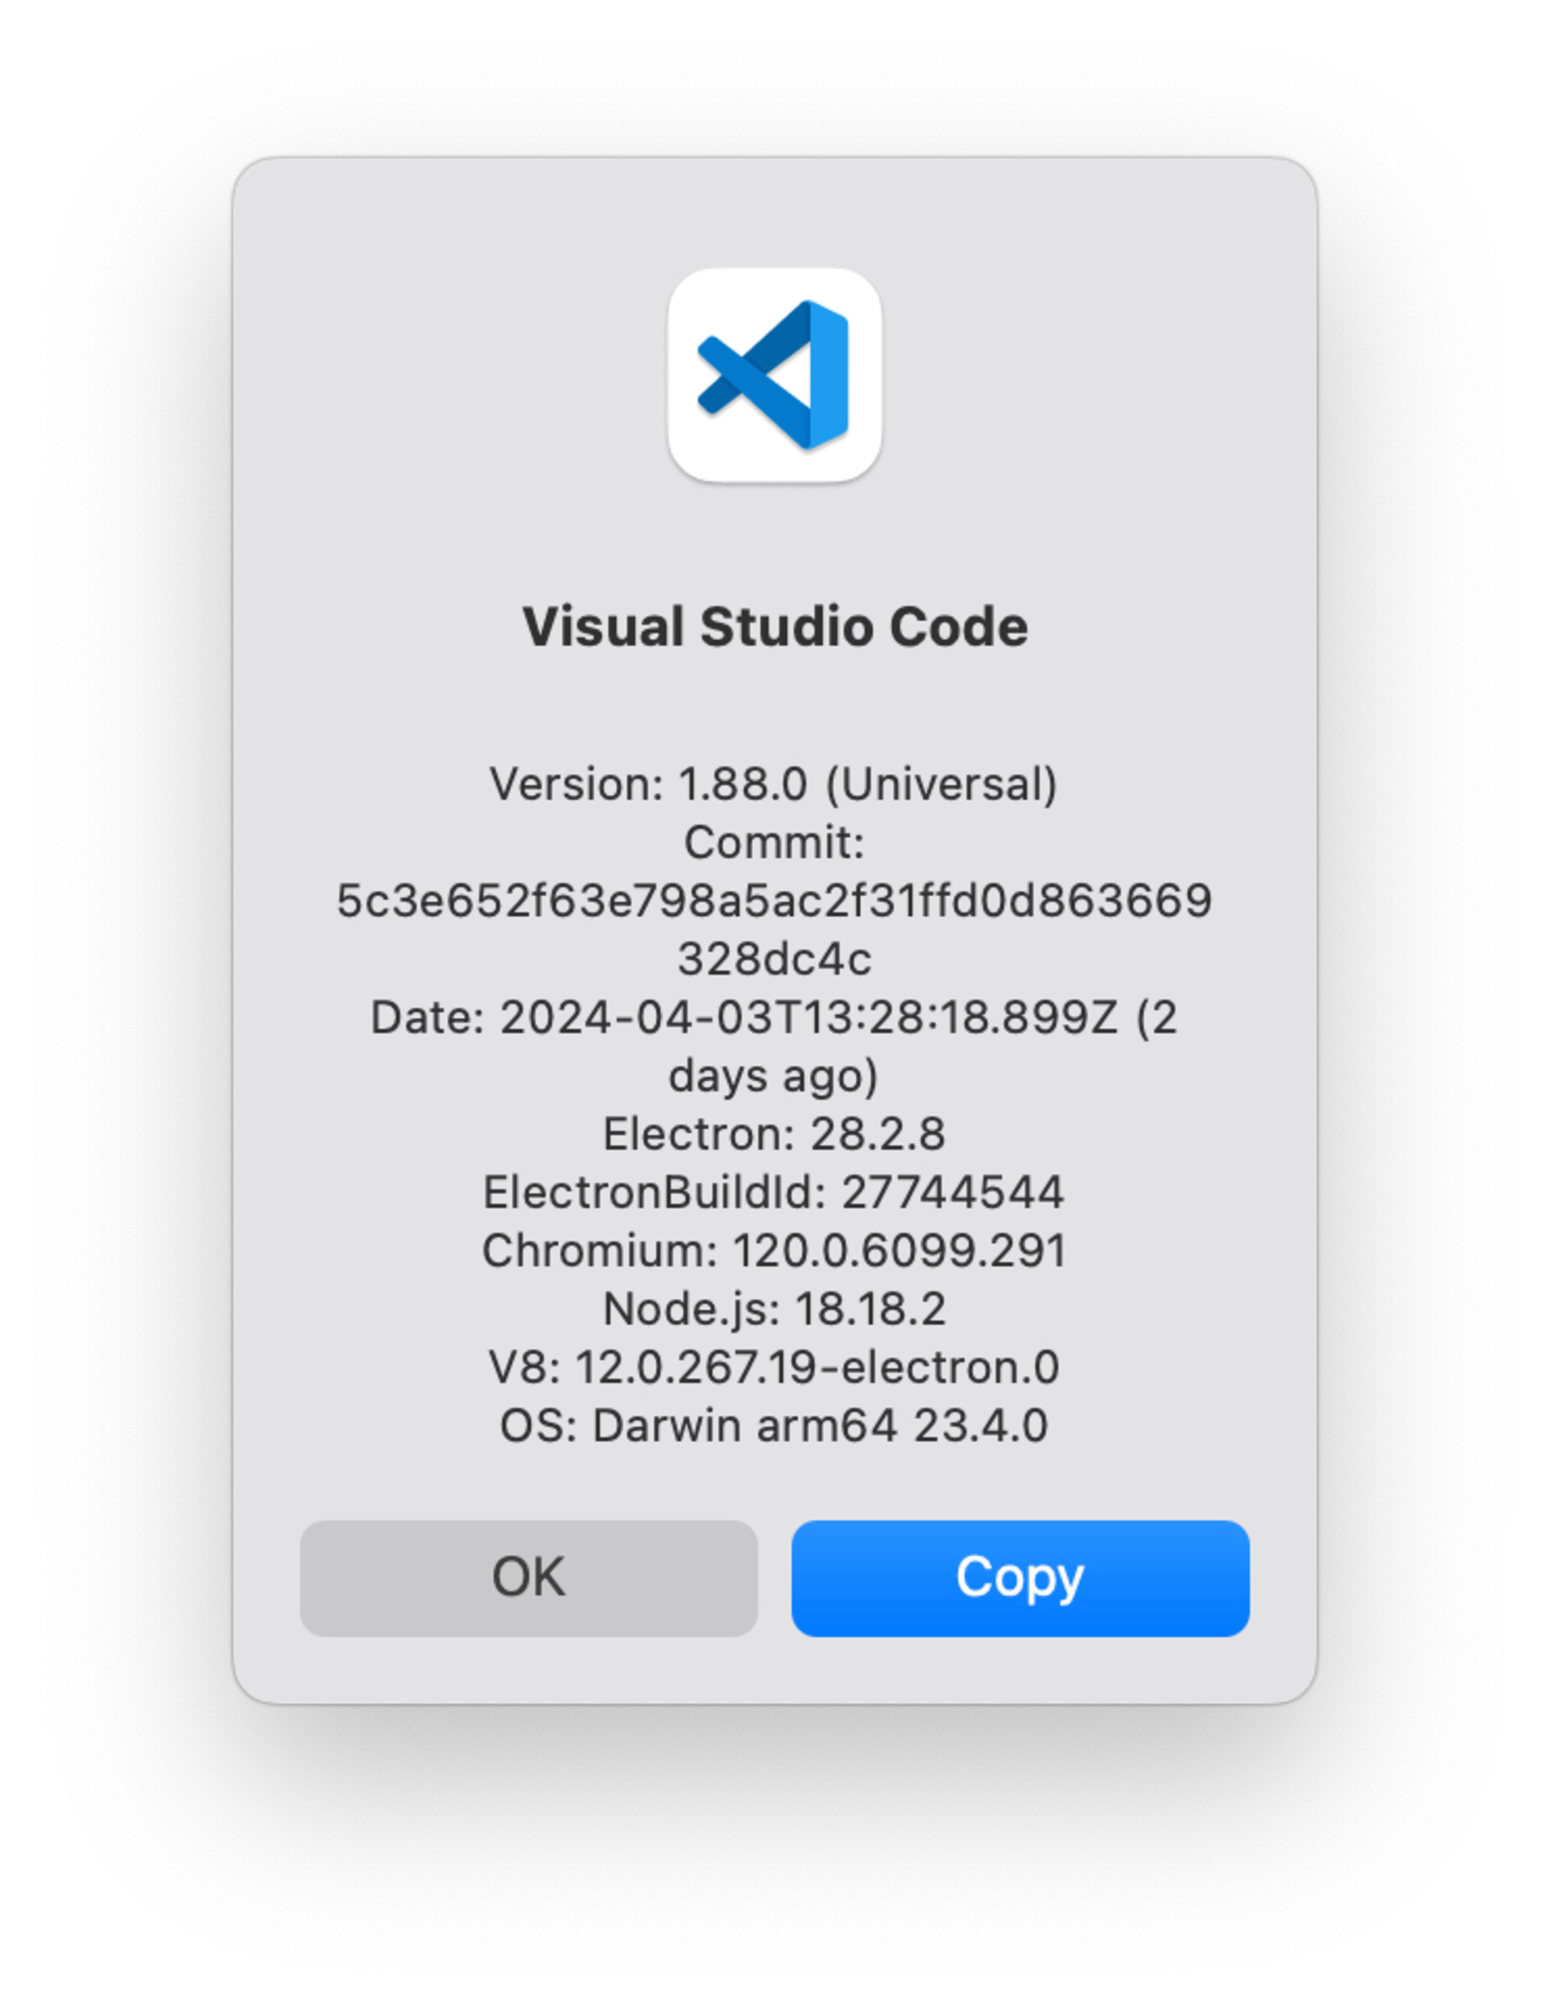
\includegraphics[width=7cm, trim=0 40  0 30, clip]{ScreenCapture4.pdf}
%\caption{}\label{vscode}
%\end{figure}
%
%\begin{thebibliography}{9}
%   \bibitem{P5}
%      松田晃一, p5.jsプログラミングガイド  改訂版, 2021, カットシステム
%   
%   \bibitem{T}
%      山田祥寛, 
%      改訂3版JavaScript本格入門, 2023, 技術評論社
%\end{thebibliography}
%
%
%\end{document}
%
%
%\section{GPUとCPU}
%
%\section{剛体的な図形の作図}



